%!TEX program = xelatex
% Note: this template must be compiled with XeLaTeX rather than PDFLaTeX
% due to the custom fonts used. The line above should ensure this happens
% automatically, but if it doesn't, your LaTeX editor should have a simple toggle
% to switch to using XeLaTeX.

\documentclass[
	aspectratio=169, % Uncomment to use an aspect ratio of 16:9 (160 mm by 90 mm)
	%aspectratio=43, % Uncomment to use an aspect ratio of 4:3 (128mm by 96mm)
	t, % Top align all slide content by default
	onlytextwidth, % Typeset content in columns at text width
	10pt, % Default font size, use 10pt for the 16:9 aspect ratio and 8pt for the 4:3 aspect ratio
]{beamer}

\usepackage{../ImperialTheme/beamerthemeImperial} % Use the Imperial theme

\def\imagefolder{../ImperialTheme/Images/}

\title{TS mode!} % Presentation title to appear on the title slide and left footers

\subtitle{} % Presentation subtitle to appear on the title slide

\author{Víctor Ballester} % Author name(s) to appear on the title slide

\date{\today} % Presentation date to appear on the title slide and right footers

\begin{document}

\begingroup
\setbeamercolor{background canvas}{bg=ICLBlue} % Slide background color
\setbeamercolor{title page title}{fg=white} % Title text color
\setbeamercolor{title page subtitle}{fg=white} % Subtitle text color
\setbeamercolor{author}{fg=white} % Author(s) text color
\setbeamercolor{date}{fg=white} % Date text color
\setbeamertemplate{title page}[logo]{\imagefolder/ICL_Logo_White.pdf} % Imperial logo color, use 'ICL_Logo_White.pdf' for white and 'ICL_Logo_Blue.pdf' for blue
\frame[plain, s]{\titlepage} % Output the title page with no footer ('plain') and vertically distributed text ('s')
\endgroup

\begin{frame}
	\frametitle{Summary}
	\begin{itemize}
		\item I ran the case with $w=16.5 \delta^*$ (remember that $w=16.35 \delta^*$ is naturally stable as $t\to\infty$).
		\item So I needed to use SFD to get a good baseflow (accurate enough, up to residuals of $10^{-6}$).
		\item Then, I ran the linearized solver to get the global modes. Interestingly, changing the number of steps for the Arnoldi iteration I got two different results. 
		\begin{itemize}
			\item With `few" steps I got the TS mode with growth rate of $-0.00543859$ and frequency of $\pm 0.0260322$.
			\item With more steps I got a greater-in-growth-rate mode, with growth rate of $-0.00258415$ and frequency of $\pm 0.00276843$. And I `showed" this is the greatest growth rate.
		\end{itemize}
	\end{itemize}
        
\end{frame}
\begin{frame}
	\frametitle{TS mode}
	{
	u component
	\centering
	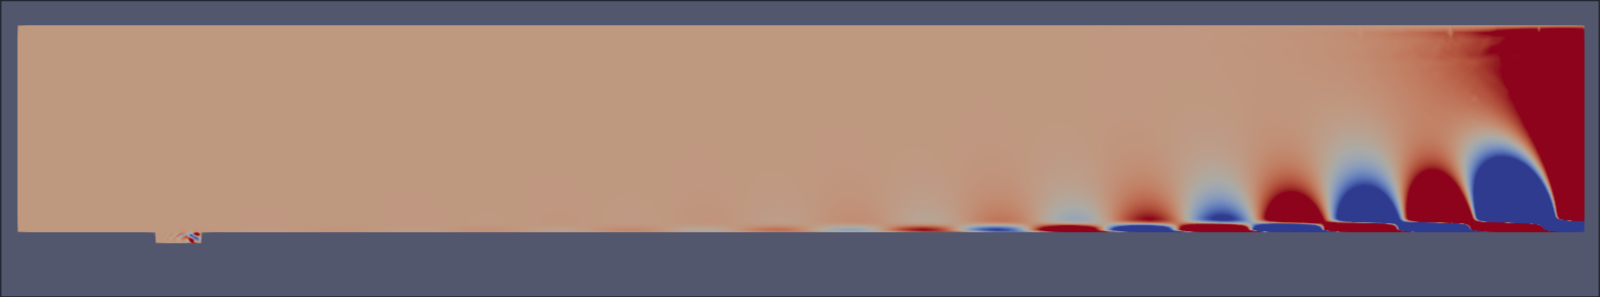
\includegraphics[width=\linewidth]{Images/TSu.png}
	v component
	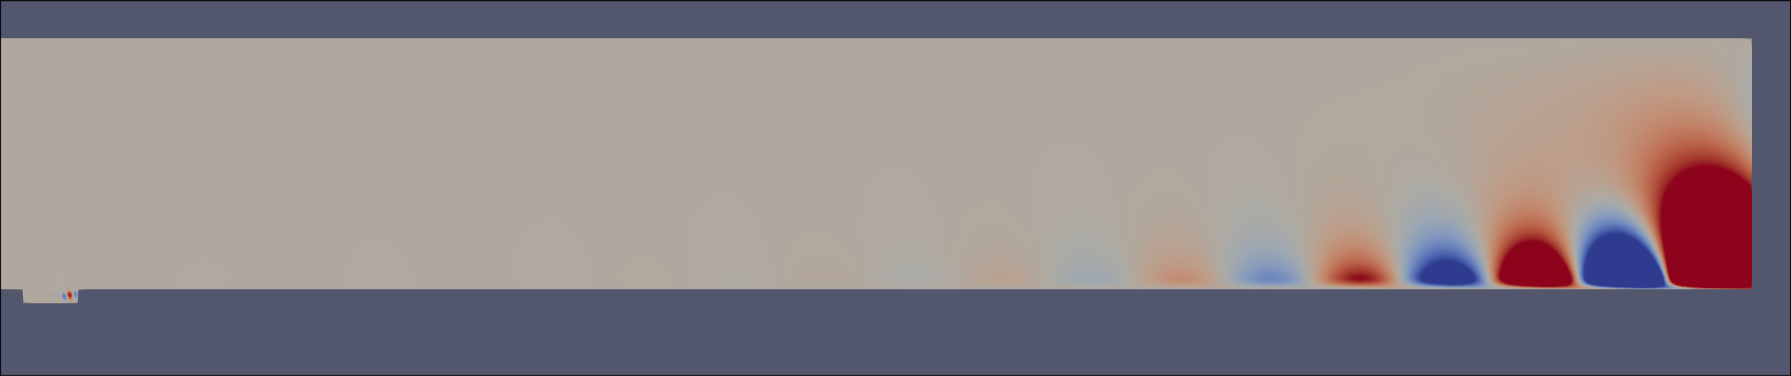
\includegraphics[width=\linewidth]{Images/TSv.png}
	}
\end{frame}
\begin{frame}
	\frametitle{TS mode}
	{
	v component
	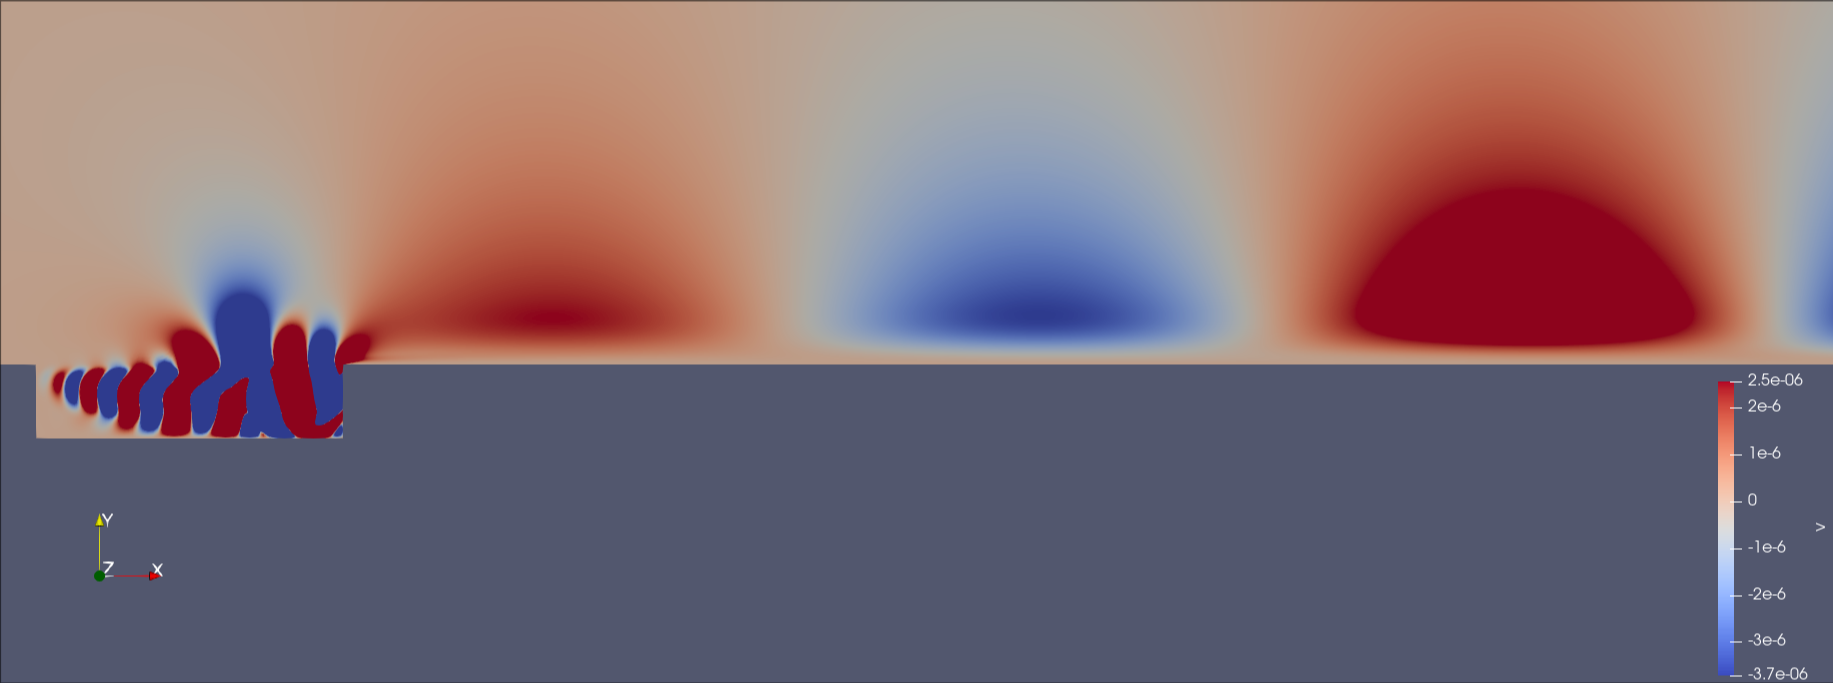
\includegraphics[width=\linewidth]{Images/zoomedTSv.png}
	}
\end{frame}

\begin{frame}
	\frametitle{Huge Mode}
	
	u component
	{
	\centering
	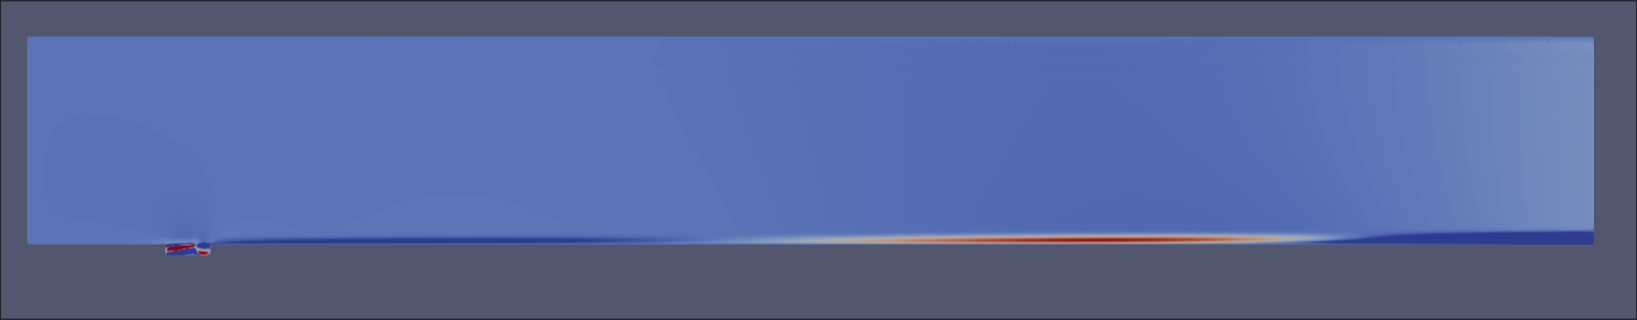
\includegraphics[width=\linewidth]{Images/HugeMode.png}
	}

\end{frame}
\begin{frame}
	\frametitle{Questions}
	\begin{itemize}
		\item What is destabilizing my system if every global mode is stable?
	\end{itemize}
	
\end{frame}
\end{document}
